\documentclass[float=false, crop=false]{standalone}
\linespread{1.3}

\usepackage[subpreambles=true]{standalone}
\usepackage{import}

\usepackage{parskip}
\setlength{\parindent}{0pt} %no paragraph indentation
\setlength{\parskip}{2.1ex plus 0.2ex minus 0.2ex} %3x paragraph spacing

\usepackage{geometry}
\geometry{letterpaper,left=1.0in,right=1.0in,top=1.0in,bottom=1.0in}

\usepackage{fancyhdr}
\pagestyle{fancy}
\fancyhf{}
\renewcommand{\headrulewidth}{0pt}
\rfoot{\thepage}

\usepackage{hyperref}

\usepackage[fleqn]{amsmath}
\usepackage{amssymb}
\usepackage{amsthm}

\usepackage{graphicx}
\graphicspath{{./imgs/}}

\begin{document}
	
	In \cite{Brenner2007} a microbial consortium was designed using a quorum-sensing mechanism for inter-cellular communication. The signaling modules \textit{lasI}/\textit{lasR} and \textit{rhlI}/\textit{rhlR} were used to regulate expressions in the consortia partner; see figure~\ref{fig:brenner2007_genecircuits}.
	
	\begin{figure}[h]
		\centering
		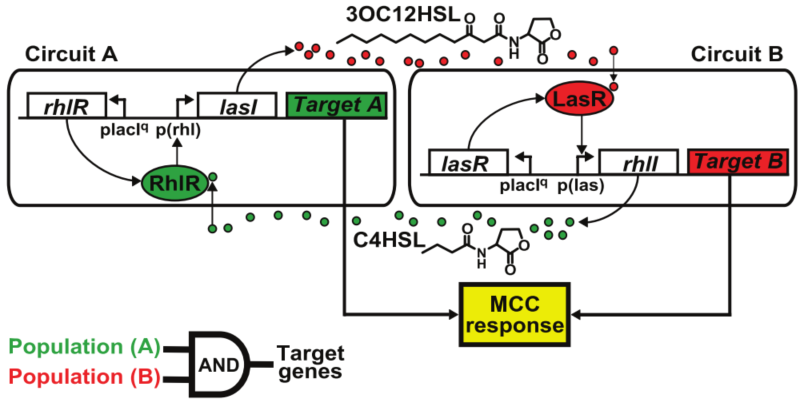
\includegraphics[width=0.8\textwidth]{brenner2007_genecircuits.png}
		\caption{Gene circuits.}
		\label{fig:brenner2007_genecircuits}
	\end{figure}	
	The authors attempted to design an AND type logic gate i.e. only if both cell densities are high should the consortium response be on. Green and red fluorescence genes were used to measure the respective response with both fluorescence proteins expressed corresponding to an on signal. The authors noted that there was some cross talk between the signaling systems e.g. high levels of one signal triggers both responses. By modeling the system dynamics it was found that a positive feedback loop attenuated this issue.
	
	The paper focuses on biofilm applications but nevertheless tests on solid and liquid media were successful. The paper also contains the differential equation models used for the planning stages.
	
	
	\ifstandalone
		\bibliographystyle{unsrt}	
		\bibliography{../../../Research/library}
	\fi

\end{document}